\chapter{First chapter}

I am fake contents of the first chapter.

\section{First section}

I am the first section.

\begin{figure}
  \centering
  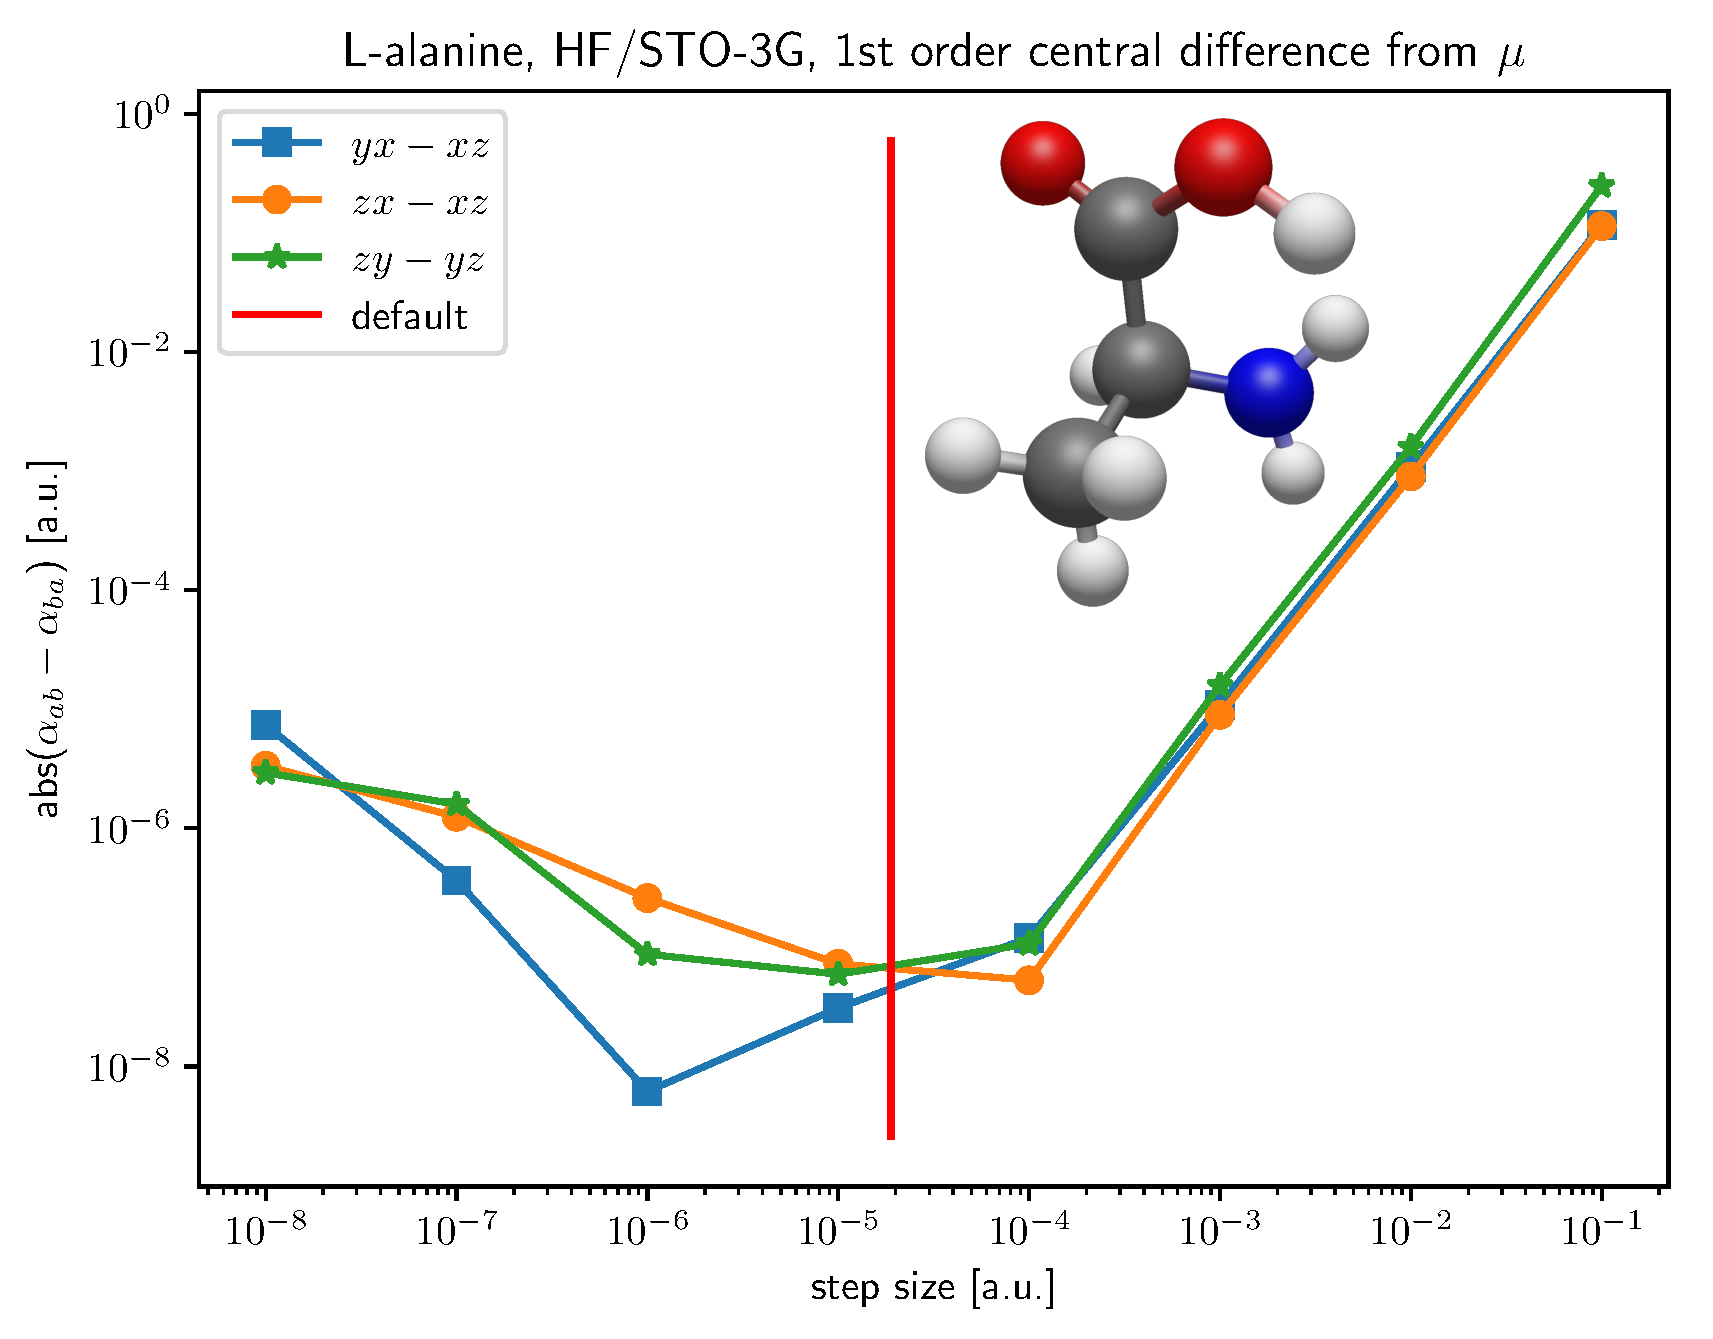
\includegraphics[width=\textwidth]{./diff_overlay.pdf}
  \caption{Asymmetry in the 1st-order finite-difference polarizability\label{fig:finite-difference-numerical-noise}}
\end{figure}

\begin{table}
  \centering
  \caption[MO coefficient derivatives and rotation matrices needed for energy derivatives]{Orders of MO coefficient derivatives and rotation matrices needed for energy derivatives following Wigner's \(2n+1\) rule. Reproduced from Ref.~\parencite{Yamaguchi1994}.}
  \label{tutorial:tab:wigner}
  \begin{tabular}{cccc}
    \toprule
    & CI: MO/CI space & MCSCF: MO/CI space & RHF: MO space \\
    \midrule
    Energy, \(E\) & \(C_{\mu}^{i}\), \(C_{I}\) & \(C_{\mu}^{i}\), \(C_{I}\) & \(C_{\mu}^{i}\) \\
    First Derivative, \(\frac{\partial E}{\partial a}\) & \(U^{a}\), \(C_{I}\) & \(C_{\mu}^{i}\), \(C_{I}\) & \(C_{\mu}^{i}\) \\
    Second Derivative, \(\frac{\partial^{2} E}{\partial a \partial b}\) & \(U^{ab}\), \(\frac{\partial C_{I}}{\partial a}\) & \(U^{a}\), \(\frac{\partial C_{I}}{\partial a}\) & \(U^{a}\) \\
    Third Derivative, \(\frac{\partial^{3} E}{\partial a \partial b \partial c}\) & \(U^{abc}\), \(\frac{\partial C_{I}}{\partial a}\) & \(U^{a}\), \(\frac{\partial C_{I}}{\partial a}\) & \(U^{a}\) \\
    Fourth Derivative, \(\frac{\partial^{4} E}{\partial a \partial b \partial c \partial d}\) & \(U^{abcd}\), \(\frac{\partial^{2} C_{I}}{\partial a \partial b}\) & \(U^{ab}\), \(\frac{\partial^{2} C_{I}}{\partial a \partial b}\) & \(U^{ab}\) \\
    Fifth Derivative, \(\frac{\partial^{5} E}{\partial a \partial b \partial c \partial d \partial e}\) & \(U^{abcde}\), \(\frac{\partial^{2} C_{I}}{\partial a \partial b}\) & \(U^{ab}\), \(\frac{\partial^{2} C_{I}}{\partial a \partial b}\) & \(U^{ab}\) \\
    \bottomrule
  \end{tabular}
\end{table}

\begin{algorithm}
  \(i,j\) are input/output node indices into the weight coefficient matrix.
  \begin{algorithmic}[1]
    \State Training set \(\gets \{ (x^{(1)},y^{(1)}), ..., (x^{(m)},y^{(m)}) \}\)
    \State \(\Delta_{ij}^{(l)} \gets 0\) for all \(l,i,j\)
    \For{training example \(t \gets 1, m\)}
      \State \(a^{(1)} \gets x^{(t)}\)
      \State Perform forward propagation to compute \(a^{(l)}\) for \(l=2,3,...,L\)
      \State \(\delta^{(L)} \gets a^{(L)} - y^{(t)}\)
      \Comment{Initialize backpropagation routine at output layer.}
      \For{\(l \gets L-2, 2\)}
        \Comment{Work backwards through layers.}
        \State \( g'(s^{(l)}) \gets a^{(l)} \odot (1 - a^{(l)}) \)
        \State \( \delta^{(l)} \gets ( (w^{(l)})^{T} \delta^{(l+1)} ) \odot g'(s^{(l)}) \)
        %% \State \( \Delta_{ij}^{(l)} \gets \Delta_{ij}^{(l)} + a_{j}^{(l)} \delta_{i}^{(l+1)} \) for all \(i,j\)
        \State \( \Delta^{(l)} \gets \Delta^{(l)} + \delta^{(l+1)} (a^{(l)})^{T}  \)
        \State \(D_{ij}^{(l)} \gets \frac{1}{m} \Delta_{ij}^{(l)} + \lambda w_{ij}^{(l)} \)
      \EndFor
    \EndFor
    \State \( \frac{\partial}{\partial w_{ij}^{(l)}} J(w) \gets D_{ij}^{(l)} \)
  \end{algorithmic}
  The regularization term with hyperparameter \(\lambda\) is set to zero if \(j = 0\) (the bias node).
  \caption{Backpropagation for computing weight updates in a fully-connected neural network}
\end{algorithm}
